%\sgcnote{Es importante explicar aca por que se trabaja con simulaciones y como se espera que estas sean representativas para su posterior validacion en terreno. Por ejemplo, puedes mencionar brevemente cosas asociadas a la pandemia, poco acceso al material, etc. Si es importante especificar que aun las simulaciones son relevantes, para que no suene como que quedo un trabajo incompleto porque se te acabo el tiempo o te dio flojera.  Tambien esto deberia ir especificado en los alcances en el capitulo 1.}

Con el fin de constatar el correcto funcionamiento del hardware diseñado en el Capítulo \ref{cap:sadq}, se realizó una evaluación experimental consistente en emular pulsos digitales de entrada mediante la implementación de un módulo de hardware auxiliar diseñado especialmente para este propósito, sumado a las herramientas de depuración disponibles en el software de desarrollo Vivado: VIO (Virtual Input/Output)\cite{XilinxVirtualSuite} e ILA (Integrated Logic Analyzer)\cite{XilinxIntegratedPG172}, contrastando así la integridad y duración de los pulsos capturados respecto a los datos recibidos por comunicación serial en un computador receptor. 

La evaluación experimental se realiza mediante emulación de pulsos digitales en el hardware implementado y no mediante pulsos reales debido al contexto de pandemia en el cual se desarrolla esta memoria de titulación, lo que implica la imposibilidad de acceder al sistema de detección real y a los equipos de laboratorio necesarios para operarlo. Se espera que esta evaluación experimental sea representativa del sistema real mediante la emulación de pulsos digitales con tiempos de duración equivalentes a los pulsos de detección reales (entre 2ns y 90ns), con un ratio de detección mayor al esperado (1 evento cada 2$\mu$s en vez de 1 por minuto) y abarcando todos los canales de captura disponibles en el sistema de adquisición implementado.

La Figura \ref{fig:emu} ilustra la ubicación e interconexión entre el sistema de adquisición y los módulos de depuración y emulación de pulsos. Los bloques en naranjo representan al módulo VIO, ILA y Módulo Auxiliar, encargados de dar inicio al experimento, monitorear las señales de entrada y salida del sistema de adquisición, y emular los pulsos digitales de detección respectivamente.

\begin{figure}[ht]
	\centering
	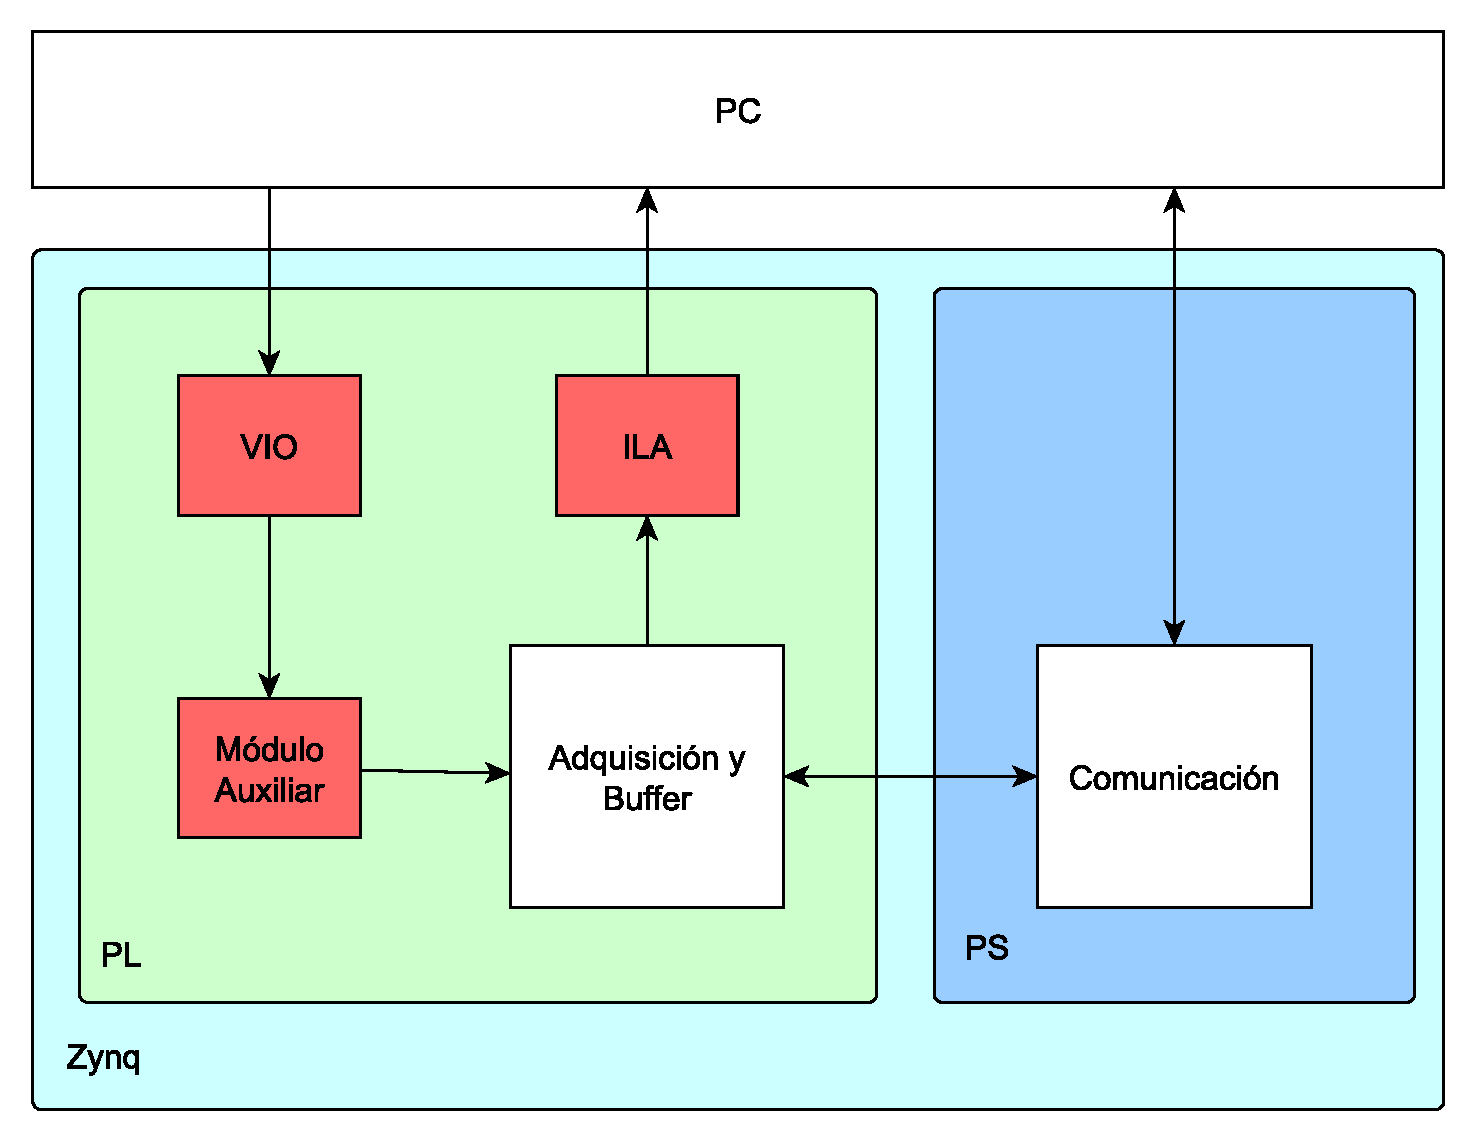
\includegraphics[scale=0.5]{emu.pdf}
	\caption{Configuración experimental para la emulación de pulsos digitales y monitoreo del sistema de adquisición implementado.}
	\label{fig:emu}
\end{figure}

El módulo auxiliar de emulación tiene como objetivo generar un exhaustivo barrido de señales abarcando todos los puertos de adquisición y emula señales equivalentes a 36 eventos de detección en diferentes vértices de interacción de un detector sTGC imaginario. Por ejemplo, la Figura \ref{img:digital_test_example} representa uno de los 36 eventos emulados, particularmente el evento 10, en donde se observan 6 canales coloreados en naranjo, correspondientes a tres canales por cada eje coordenado. En el centro de la intersección de canales coloreada en verde se encuentra el vértice de interacción estimado (coloreado en celeste). Cada evento representa un vértice de adquisición diferente y excita siempre 3 puertos de adquisición por cada eje coordenado, lo que se traduce a 36 diferentes combinaciones de señales para la representación de los eventos de prueba. Además, la duración de las señales es diferente en cada evento, partiendo con 36 ciclos de reloj de duración para las señales del primer evento y terminando con 1 ciclo de reloj de duración para las señales del último evento enviado, logrando así poner a prueba la resolución temporal del sistema de adquisición.
	
	\begin{figure}[h]
		\centering
		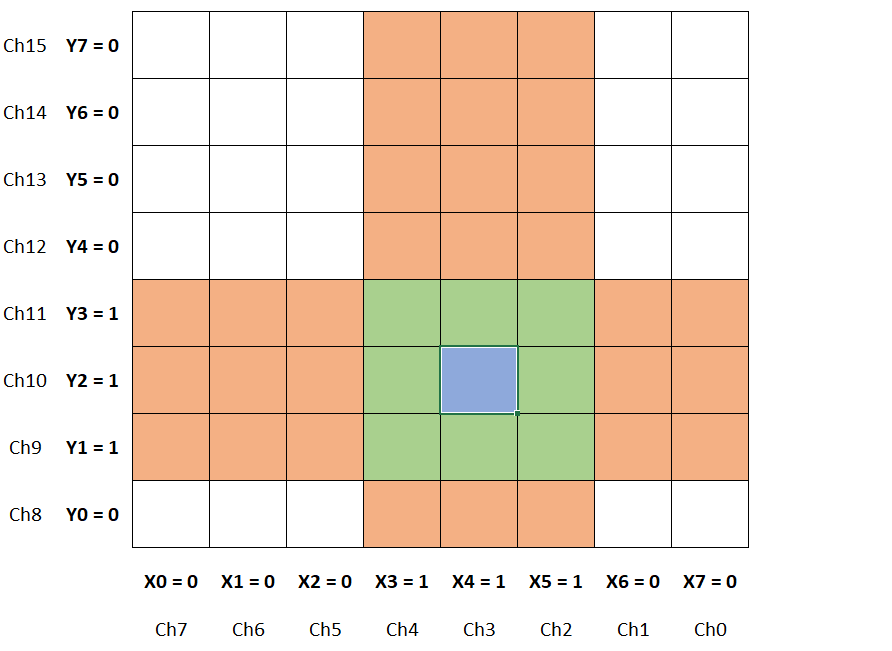
\includegraphics[scale=0.65]{digital_test_example.png}
		\caption{Ejemplo de uno de los 36 eventos, correspondiente al evento de prueba número 10. }
		\label{img:digital_test_example}
	\end{figure}
	
	El envío de los 36 eventos se inició mediante un botón virtual configurado en un bloque VIO, mientras que las señales internas se monitorearon con un bloque ILA. Los datos generados por el sistema de adquisición diseñado fueron leídos a través de una consola serial incluida en la interfaz del software Xilinx SDK 2019.1. Las Figuras \ref{img:e1} y \ref{img:e4} corresponden a capturas de pantalla de la interfaz ILA e ilustran las señales internas asociadas a los eventos 1 y 4 respectivamente. En ambas figuras se incluyen 6 señales: \textit{Start\_bttn}, correspondiente a la señal emitida por el botón configurado en la VIO; \textit{Input\_Event}, vector de 15bits que representa los datos enviados desde el módulo auxiliar hacia el sistema de adquisición; \textit{Trigger}, correspondiente a la emulación de una señal de disparo con un delay de 48 ciclos de reloj; la señal para habilitar la escritura en la memoria FIFO, nombrada como \textit{FIFO\_write\_enable}; \textit{FIFO\_data\_input}, vector de 64bits asociado a los datos recibidos por el sistema de adquisición listos para ser guardados en la memoria FIFO; y \textit{FIFO\_empty\_flag}, la cual corresponde a la señal emitida por la memoria FIFO cuando está vacía.
	
	En la Figura \ref{img:e1} se ilustran las señales internas asociadas al primer evento enviado y se sitúan en ella 4 marcadores azules y un marcador verde. Los primeros dos marcadores azules corresponden al inicio y término del envío de señales a través del vector \textit{Input\_event}, indicando que la duración de este grupo de señales es de 9 ciclos de reloj. Dado que la frecuencia de reloj utilizada para el bloque ILA es de 100MHz, pero el módulo auxiliar opera a 400MHz, se tiene entonces que la duración de las señales emitidas correspondientes al primer evento es 4 veces la cantidad de ciclos demarcada, significando una duración de 36 ciclos (90ns) para este evento. Así se comprueba que la señal ha sido correctamente emitida. Además su valor en notación hexadecimal corresponde a \texttt{0x07e0}, que se traduce en binario a \texttt{0b0000011111100000} y representa que los canales excitados corresponden a los primeros 3 de cada eje coordenado.  %\sgcnote{Revisa bien la escritura de todo este capitulo. Hay varios typos de puntuacion, tildes, y demases.}
	
	Los últimos dos marcadores azules de la Figura \ref{img:e1} demarcan el inicio y término de la escritura en memoria (\textit{FIFO\_write\_enable}) de los datos capturados por el sistema de adquisición. Este proceso de escritura toma 16 ciclos de reloj, que efectivamente corresponden a los 16 ciclos necesarios para escribir la información de cada uno de los 16 canales capturados por el sistema de adquisición según el reloj de 100MHz asociado a la memoria FIFO. El marcador verde está situado en medio de la información a ser escrita en la memoria FIFO indicada por el vector de 64 bits \textit{FIFO\_data\_input}, donde se puede observar el número hexadecimal \texttt{0x1FFFFFFFFE} que representa la duración de los 6 canales intermedios excitados por este evento. Sumando el número de bits en alto que contiene este dato hexadecimal se obtiene 36, lo que corresponde a la los ciclos de reloj que dura el evento 1.
	
	La señal \textit{trigger} indicada en la Figura \ref{img:e1} no es observable debido a la frecuencia de reloj del analizador lógico, la cual es 4 veces más lenta que el reloj al que opera la emisión y captura de pulsos de disparo. En la Figura \ref{img:e4} sí es posible observar la señal de disparo ya que corresponde al cuarto evento enviado por el módulo auxiliar, por ser múltiplo de 4. En esta figura se observa una señal de disparo correspondiente a 12 ciclos de reloj del analizador lógico, que se traducen a 48 ciclos de reloj en el dominio de la adquisición de datos y equivale a un retardo de 120ns respecto a la emisión del evento representado en la Figura \ref{img:e4}.
	
	\begin{figure}[ht]
		\centering
		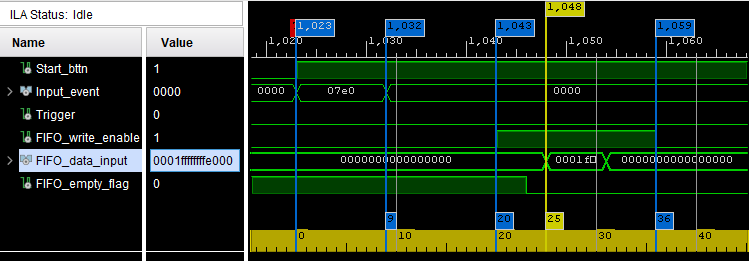
\includegraphics[scale=0.7]{e1.png}
		\caption{Captura de pantalla de la interfaz ILA, donde se ilustra la recepción del primer evento de prueba.}
		\label{img:e1}
	\end{figure}
	
	
	\begin{figure}[ht]
		\centering
		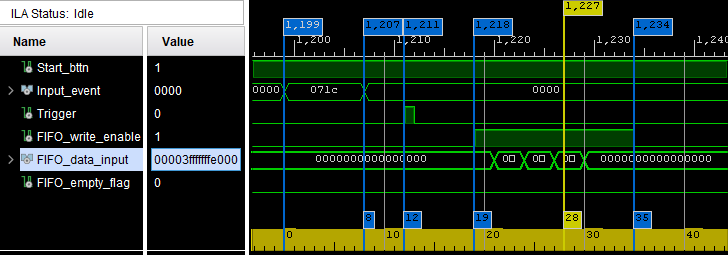
\includegraphics[scale=0.7]{e4.png}
		\caption{Captura de pantalla de la interfaz ILA, donde se ilustra la recepción del cuarto evento de prueba.}
		\label{img:e4}
	\end{figure}

	Finalmente, se realizó este experimento 28 veces consecutivas sin ninguna variabilidad sumando un total de 1008 eventos capturados con la misma secuencia y duración de señales, para así comparar y comprobar que los eventos con \textit{glitches} o errores de medición sean menores al 1\% del total de eventos y no interfieran en el posterior análisis e interpretación de los eventos detectados. Dado que la generación de una muongrafía requiere analizar miles de eventos, contar con menos del 1\% de eventos defectuosos no tiene mayores repercusiones y se considera despreciable. En cuanto al muestreo del tiempo de duración de cada señal, se espera que el error no sea mayor a $\pm$2,5ns, correspondiente a la resolución temporal del sistema de adquisición diseñado. %\sgcnote{se hizo exactamente el mismo experimento 28 veces? Hubo alguna variabilidad? Que tan representativo/concluyente es esto? }. 
	
	Durante la prueba experimental, los eventos emulados fueron recepcionados mediante comunicación serial y fueron analizados a través de un programa para contar los bits contenidos en cada canal de cada evento. El conteo de bits se realizó con el algoritmo de Brian Kernighan\cite{SinghCountC++} para conteo de bits en números enteros. Así se comprobó que para los 1008 eventos se logró capturar la totalidad de las señales emuladas y se pudo muestrear correctamente el 100\% de la duración de cada señal con una resolución temporal de 2,5ns. El programa utilizado y los archivos generados en la adquisición de eventos se encuentran disponibles en el repositorio de este proyecto \cite{GonzalezMuonRepository}. La Tabla \ref{tab:datos-serial} corresponde a los datos obtenidos por comunicación serial ya procesados mediante el algoritmo para conteo de bits y representa la duración de cada evento en ciclos de reloj, considerando un reloj de 400MHz.	
	
	Los resultados de esta prueba fueron satisfactorios, ya que no hubieron errores ni en la medición ni en la transferencia de los eventos emulados, alcanzando un 0\% de eventos defectuosos y 0ns de error en el muestreo de señales.
	La baja tasa de eventos defectuosos comprueba el correcto funcionamiento del sistema de adquisición de datos en cuanto a su resolución, lógica de operación y módulos de comunicación para la adquisición de pulsos digitales sincrónicos. Cabe mencionar que para eventos reales las tasas de error serán mayores debido a la incidencia de señales con duraciones menores a la resolución máxima disponible de 2,5ns, además de la posible existencia de errores de detección, disparo y transferencia de señales provenientes del sistema de detección, los cuales no están considerados en esta prueba experimental y contribuirían a aumentar el porcentaje de error global de sTGC Minería. Ambas desventajas hacen necesaria la realización de pruebas experimentales que incluyan los sistemas reales de detección y disparo para realizar una caracterización completa del sistema y determinar así porcentajes de error globales, pero con la seguridad de que el sistema de adquisición es capaz de muestrear completamente aquellas señales que estén dentro de su rango de muestreo.
	
	\begin{table}[ht]
		\centering
		\resizebox{\textwidth}{!}{%
			\begin{tabular}{|l|r|r|r|r|r|r|r|r|r|r|r|r|r|r|r|r|}
				\hline
				\rowcolor[HTML]{70AD47} 
				{\color[HTML]{FFFFFF} \textbf{Evento}} &
				\multicolumn{1}{l|}{\cellcolor[HTML]{70AD47}{\color[HTML]{FFFFFF} \textbf{Ch0}}} &
				\multicolumn{1}{l|}{\cellcolor[HTML]{70AD47}{\color[HTML]{FFFFFF} \textbf{Ch1}}} &
				\multicolumn{1}{l|}{\cellcolor[HTML]{70AD47}{\color[HTML]{FFFFFF} \textbf{Ch2}}} &
				\multicolumn{1}{l|}{\cellcolor[HTML]{70AD47}{\color[HTML]{FFFFFF} \textbf{Ch3}}} &
				\multicolumn{1}{l|}{\cellcolor[HTML]{70AD47}{\color[HTML]{FFFFFF} \textbf{Ch4}}} &
				\multicolumn{1}{l|}{\cellcolor[HTML]{70AD47}{\color[HTML]{FFFFFF} \textbf{Ch5}}} &
				\multicolumn{1}{l|}{\cellcolor[HTML]{70AD47}{\color[HTML]{FFFFFF} \textbf{Ch6}}} &
				\multicolumn{1}{l|}{\cellcolor[HTML]{70AD47}{\color[HTML]{FFFFFF} \textbf{Ch7}}} &
				\multicolumn{1}{l|}{\cellcolor[HTML]{70AD47}{\color[HTML]{FFFFFF} \textbf{Ch8}}} &
				\multicolumn{1}{l|}{\cellcolor[HTML]{70AD47}{\color[HTML]{FFFFFF} \textbf{Ch9}}} &
				\multicolumn{1}{l|}{\cellcolor[HTML]{70AD47}{\color[HTML]{FFFFFF} \textbf{Ch10}}} &
				\multicolumn{1}{l|}{\cellcolor[HTML]{70AD47}{\color[HTML]{FFFFFF} \textbf{Ch11}}} &
				\multicolumn{1}{l|}{\cellcolor[HTML]{70AD47}{\color[HTML]{FFFFFF} \textbf{Ch12}}} &
				\multicolumn{1}{l|}{\cellcolor[HTML]{70AD47}{\color[HTML]{FFFFFF} \textbf{Ch13}}} &
				\multicolumn{1}{l|}{\cellcolor[HTML]{70AD47}{\color[HTML]{FFFFFF} \textbf{Ch14}}} &
				\multicolumn{1}{l|}{\cellcolor[HTML]{70AD47}{\color[HTML]{FFFFFF} \textbf{Ch15}}} \\ \hline
				\rowcolor[HTML]{E2EFDA} 
				\textbf{1}  & 0  & 0  & 0  & 0  & 0  & 36 & 36 & 36 & 36 & 36 & 36 & 0  & 0  & 0  & 0  & 0 \\ \hline
				\rowcolor[HTML]{FFFFFF} 
				\textbf{2}  & 0  & 0  & 0  & 0  & 35 & 35 & 35 & 0  & 35 & 35 & 35 & 0  & 0  & 0  & 0  & 0 \\ \hline
				\rowcolor[HTML]{E2EFDA} 
				\textbf{3}  & 0  & 0  & 0  & 34 & 34 & 34 & 0  & 0  & 34 & 34 & 34 & 0  & 0  & 0  & 0  & 0 \\ \hline
				\rowcolor[HTML]{FFFFFF} 
				\textbf{4}  & 0  & 0  & 33 & 33 & 33 & 0  & 0  & 0  & 33 & 33 & 33 & 0  & 0  & 0  & 0  & 0 \\ \hline
				\rowcolor[HTML]{E2EFDA} 
				\textbf{5}  & 0  & 32 & 32 & 32 & 0  & 0  & 0  & 0  & 32 & 32 & 32 & 0  & 0  & 0  & 0  & 0 \\ \hline
				\rowcolor[HTML]{FFFFFF} 
				\textbf{6}  & 31 & 31 & 31 & 0  & 0  & 0  & 0  & 0  & 31 & 31 & 31 & 0  & 0  & 0  & 0  & 0 \\ \hline
				\rowcolor[HTML]{E2EFDA} 
				\textbf{7}  & 0  & 0  & 0  & 0  & 0  & 30 & 30 & 30 & 0  & 30 & 30 & 30 & 0  & 0  & 0  & 0 \\ \hline
				\rowcolor[HTML]{FFFFFF} 
				\textbf{8}  & 0  & 0  & 0  & 0  & 29 & 29 & 29 & 0  & 0  & 29 & 29 & 29 & 0  & 0  & 0  & 0 \\ \hline
				\rowcolor[HTML]{E2EFDA} 
				\textbf{9}  & 0  & 0  & 0  & 28 & 28 & 28 & 0  & 0  & 0  & 28 & 28 & 28 & 0  & 0  & 0  & 0 \\ \hline
				\rowcolor[HTML]{FFFFFF} 
				\textbf{10} & 0  & 0  & 27 & 27 & 27 & 0  & 0  & 0  & 0  & 27 & 27 & 27 & 0  & 0  & 0  & 0 \\ \hline
				\rowcolor[HTML]{E2EFDA} 
				\textbf{11} & 0  & 26 & 26 & 26 & 0  & 0  & 0  & 0  & 0  & 26 & 26 & 26 & 0  & 0  & 0  & 0 \\ \hline
				\rowcolor[HTML]{FFFFFF} 
				\textbf{12} & 25 & 25 & 25 & 0  & 0  & 0  & 0  & 0  & 0  & 25 & 25 & 25 & 0  & 0  & 0  & 0 \\ \hline
				\rowcolor[HTML]{E2EFDA} 
				\textbf{13} & 0  & 0  & 0  & 0  & 0  & 24 & 24 & 24 & 0  & 0  & 24 & 24 & 24 & 0  & 0  & 0 \\ \hline
				\rowcolor[HTML]{FFFFFF} 
				\textbf{14} & 0  & 0  & 0  & 0  & 23 & 23 & 23 & 0  & 0  & 0  & 23 & 23 & 23 & 0  & 0  & 0 \\ \hline
				\rowcolor[HTML]{E2EFDA} 
				\textbf{15} & 0  & 0  & 0  & 22 & 22 & 22 & 0  & 0  & 0  & 0  & 22 & 22 & 22 & 0  & 0  & 0 \\ \hline
				\rowcolor[HTML]{FFFFFF} 
				\textbf{16} & 0  & 0  & 21 & 21 & 21 & 0  & 0  & 0  & 0  & 0  & 21 & 21 & 21 & 0  & 0  & 0 \\ \hline
				\rowcolor[HTML]{E2EFDA} 
				\textbf{17} & 0  & 20 & 20 & 20 & 0  & 0  & 0  & 0  & 0  & 0  & 20 & 20 & 20 & 0  & 0  & 0 \\ \hline
				\rowcolor[HTML]{FFFFFF} 
				\textbf{18} & 19 & 19 & 19 & 0  & 0  & 0  & 0  & 0  & 0  & 0  & 19 & 19 & 19 & 0  & 0  & 0 \\ \hline
				\rowcolor[HTML]{E2EFDA} 
				\textbf{19} & 0  & 0  & 0  & 0  & 0  & 18 & 18 & 18 & 0  & 0  & 0  & 18 & 18 & 18 & 0  & 0 \\ \hline
				\rowcolor[HTML]{FFFFFF} 
				\textbf{20} & 0  & 0  & 0  & 0  & 17 & 17 & 17 & 0  & 0  & 0  & 0  & 17 & 17 & 17 & 0  & 0 \\ \hline
				\rowcolor[HTML]{E2EFDA} 
				\textbf{21} & 0  & 0  & 0  & 16 & 16 & 16 & 0  & 0  & 0  & 0  & 0  & 16 & 16 & 16 & 0  & 0 \\ \hline
				\rowcolor[HTML]{FFFFFF} 
				\textbf{22} & 0  & 0  & 15 & 15 & 15 & 0  & 0  & 0  & 0  & 0  & 0  & 15 & 15 & 15 & 0  & 0 \\ \hline
				\rowcolor[HTML]{E2EFDA} 
				\textbf{23} & 0  & 14 & 14 & 14 & 0  & 0  & 0  & 0  & 0  & 0  & 0  & 14 & 14 & 14 & 0  & 0 \\ \hline
				\rowcolor[HTML]{FFFFFF} 
				\textbf{24} & 13 & 13 & 13 & 0  & 0  & 0  & 0  & 0  & 0  & 0  & 0  & 13 & 13 & 13 & 0  & 0 \\ \hline
				\rowcolor[HTML]{E2EFDA} 
				\textbf{25} & 0  & 0  & 0  & 0  & 0  & 12 & 12 & 12 & 0  & 0  & 0  & 0  & 12 & 12 & 12 & 0 \\ \hline
				\rowcolor[HTML]{FFFFFF} 
				\textbf{26} & 0  & 0  & 0  & 0  & 11 & 11 & 11 & 0  & 0  & 0  & 0  & 0  & 11 & 11 & 11 & 0 \\ \hline
				\rowcolor[HTML]{E2EFDA} 
				\textbf{27} & 0  & 0  & 0  & 10 & 10 & 10 & 0  & 0  & 0  & 0  & 0  & 0  & 10 & 10 & 10 & 0 \\ \hline
				\rowcolor[HTML]{FFFFFF} 
				\textbf{28} & 0  & 0  & 9  & 9  & 9  & 0  & 0  & 0  & 0  & 0  & 0  & 0  & 9  & 9  & 9  & 0 \\ \hline
				\rowcolor[HTML]{E2EFDA} 
				\textbf{29} & 0  & 8  & 8  & 8  & 0  & 0  & 0  & 0  & 0  & 0  & 0  & 0  & 8  & 8  & 8  & 0 \\ \hline
				\rowcolor[HTML]{FFFFFF} 
				\textbf{30} & 7  & 7  & 7  & 0  & 0  & 0  & 0  & 0  & 0  & 0  & 0  & 0  & 7  & 7  & 7  & 0 \\ \hline
				\rowcolor[HTML]{E2EFDA} 
				\textbf{31} & 0  & 0  & 0  & 0  & 0  & 6  & 6  & 6  & 0  & 0  & 0  & 0  & 0  & 6  & 6  & 6 \\ \hline
				\rowcolor[HTML]{FFFFFF} 
				\textbf{32} & 0  & 0  & 0  & 0  & 5  & 5  & 5  & 0  & 0  & 0  & 0  & 0  & 0  & 5  & 5  & 5 \\ \hline
				\rowcolor[HTML]{E2EFDA} 
				\textbf{33} & 0  & 0  & 0  & 4  & 4  & 4  & 0  & 0  & 0  & 0  & 0  & 0  & 0  & 4  & 4  & 4 \\ \hline
				\rowcolor[HTML]{FFFFFF} 
				\textbf{34} & 0  & 0  & 3  & 3  & 3  & 0  & 0  & 0  & 0  & 0  & 0  & 0  & 0  & 3  & 3  & 3 \\ \hline
				\rowcolor[HTML]{E2EFDA} 
				\textbf{35} & 0  & 2  & 2  & 2  & 0  & 0  & 0  & 0  & 0  & 0  & 0  & 0  & 0  & 2  & 2  & 2 \\ \hline
				\rowcolor[HTML]{FFFFFF} 
				\textbf{36} & 1  & 1  & 1  & 0  & 0  & 0  & 0  & 0  & 0  & 0  & 0  & 0  & 0  & 1  & 1  & 1 \\ \hline
			\end{tabular}%
		}
		\caption{Ejemplo de tabla de datos recibida por comunicación serial, correspondiente al experimento número 15. Los números representan la duración de cada señal en ciclos de reloj de 400MHz.}
		\label{tab:datos-serial}
	\end{table}
